 \documentclass[12pt]{article}
\usepackage[utf8]{inputenc}
\usepackage{amsmath}
\usepackage{amssymb}
\usepackage[english]{babel}
\usepackage[margin = 1.2 in]{geometry}
\usepackage{wrapfig}
\usepackage{enumitem}
\usepackage{caption}
\usepackage{csquotes}
\usepackage{xcolor}
\usepackage{graphicx} 
\usepackage{subfig}
\usepackage[labelfont=bf]{caption}
\usepackage{biblatex}
\addbibresource{bibliography.bib}
\renewcommand*{\bibfont}{\large}

\begin{document}
\begin{titlepage}
    \begin{center}
        \vspace*{1cm}
        \Large
        Final Project 
        
        \vspace{0.5cm}
        
        \LARGE
        \textbf{Analysis of compartmental models in simulating the progression of the COVID-19 disease}
        \vspace{0.5cm}
        
        \Large
        SI1336 Simulation and modelling \\

        \vfill 
        Raymond Wang \\
        December 18, 2020
    \end{center}
\end{titlepage}

\thispagestyle{plain}
\Large
\begin{center}
    \Large
    \vspace{0.9cm}
    \textbf{Abstract}
\end{center}

\noindent 
\large
Compartmental models in epidemiology are the mathematical frameworks wherein the progression of infectious diseases can be modeled after, in particular the COVID-19 pandemic which has been ongoing since the writing of this report. Computer models approximate reality and a qualitative one may be of great use for policymakers in implementing preventive measures. The aim of this study, therefore, is to assess two variants of basic compartmental models and their ability in predicting the progression of COVID-19 in various situations, as well as their applicabilities and constraints.
\vspace{0.2cm}
\newline 
\indent \textbf{Key words:} Mathematical modelling, epidemiology, computational biology, simulation, data science, COVID-19, research, public health


\newpage 

\tableofcontents

\newpage 

\section{Introduction}
\subsection{Background}
As of the writing of this report, the COVID-19 disease has been permeating through all corners of the world, causing major disruptions and a devastating pandemic. To alleviate the implementation of preventive measures, policymakers must rely heavily on scientific advice and in this case, computer modeling can be extensively and effectively utilized in predicting the spread of the disease amongst populations.
\subsection{Compartmental models in epidemiology}
Compartmental models in epidemiology are the mathematical frameworks wherein the progression of infectious diseases can be modeled, utilizing a system of ordinary differential equations with various epidemiological parameters \cite{söder}. The population is classified into various segments, simulating the course of the infection of an individual.
\subsection{Epidemic SIR-model}
The epidemic SIR-model omits vital dynamics (birth and death) and categorizes the population into the segments of \textbf{S}usceptible, \textbf{I}nfected and \textbf{R}ecovered
as well as N being the sample population. The model is expressed by the following system of differential equations:
\begin{align}
\frac{dS}{dt} = - \frac{\beta I S}{N} \;, \qquad
\frac{dI}{dt} = \frac{\beta I S}{N}- \gamma I \; \qquad
\frac{dR}{dt} = \gamma I \;,
\end{align}
\noindent where $\beta$ and $\gamma$ denote the transmission and recovery rates respectively.
\subsection{SEIR-model}
For a number of infectious diseases and COVID-19 in particular, the pathogen undergoes a long-lasting incubation period wherein the infected individual has a low infectivity rate. In this case, an additional segment, \textbf{E}xposed is introduced.

\newpage 
\noindent 
The system of differential equations of this model summarizes to:
\begin{gather}
\frac{dS}{dt} = - \frac{\beta I S}{N} \;, \qquad
\frac{dE}{dt} = \frac{\beta I S}{N}- \alpha E \;, \\
\frac{dI}{dt} = \alpha E - \gamma I \;, \qquad 
\frac{dR}{dt} = \gamma I \;,
\end{gather}

\noindent where $\beta$, $\gamma$ and $\alpha$ denote the transmission,  recovery and infection rates respectively \cite{gill}.

\subsection{SIS-model}
The SIS-model aims to simulate the progression for infections with long-lasting immunity and thus the R-segment is omitted. Although this does not apply for COVID-19, it will later come to great use. The system of differential equations summarizes to:
\begin{align}
\frac{dS}{dt} = - \frac{\beta I S}{N} \;, \qquad
\frac{dI}{dt} = \frac{\beta I S}{N}- \gamma I \;, 
\end{align}
with the same definition for parameters as in the SIR-model.

\subsection{Aims and objectives}
The aim of this report is to study and compare the epidemic SIR and SEIR compartmental models in predicting the progression of the COVID-19 disease in different scenarios, with the population of Sweden being used as a reference. Two numerical integrators and their quality in modelling the compartmental models will furthermore be studied.

\newpage 
\section{Methods}
\subsection{Numerical integrators}
Being systems of differential equations, the SIR and SEIR models can be solved utilizing various numerical methods. In this case the fourth-order Runge-Kutta method and \textit{odeint} from the Scipy module in Python will be utilized and studied. 
With the fourth-order Runge-Kutta method being of order accuracy $O(h^5)$, it should in principle yield qualitative approximations of the exact solutions, and being more exact for smaller step sizes. Also, since the analytical solution for the SIS-model is widely accepted and easily derivable \cite{söder}, it has been utilized for extrapolating the quality of the numerical integrators. Nonetheless, \textit{odeint} was utilized for the ensuing simulations, and the rationale behind it is explained in section 4.5. Python coupled with Matplotlib, Numpy, Scipy etc. are to be utilized.
\subsection{Initial conditions}
As previously mentioned, the population of Sweden will be utilized as the sample size N, and is numbered at 10 373 225 individuals as of September 2020 \cite{Scb}. At the beginning of the pandemic and until now, almost none is immune to the disease which implies that everyone is susceptible. Also, assume that there is a trace of infection in the population at e.g. 8 individuals \cite{smith_moore}. This yields initial values: 
\begin{equation}
S(0) = N, \; E(0) = 0, \; I(0) = 8, \; R(0) = 0
\end{equation}
For the parameters:
\begin{itemize}
  \item $\alpha = 1/5.2$ to reflect a 5.2 day average incubation period \cite{atkeson}.
  \item $\beta = R_0 \gamma$ to match the COVID-19 reproduction number of $R_0 = 2-5$ \newline (No social distancing) \cite{sanche}. 
  \item $\gamma = 1/18$ to match an average illness duration of 18 days \cite{atkeson}.
\end{itemize}
Variations are implemented in order to simulate different scenarios.
\newpage 
\section{Results}
\subsection{Epidemic SIR - Comparisons for $R_0$-rates}
\begin{figure*}[ht!]
\begin{center}
   \subfloat[\label{genworkflow}]{%
      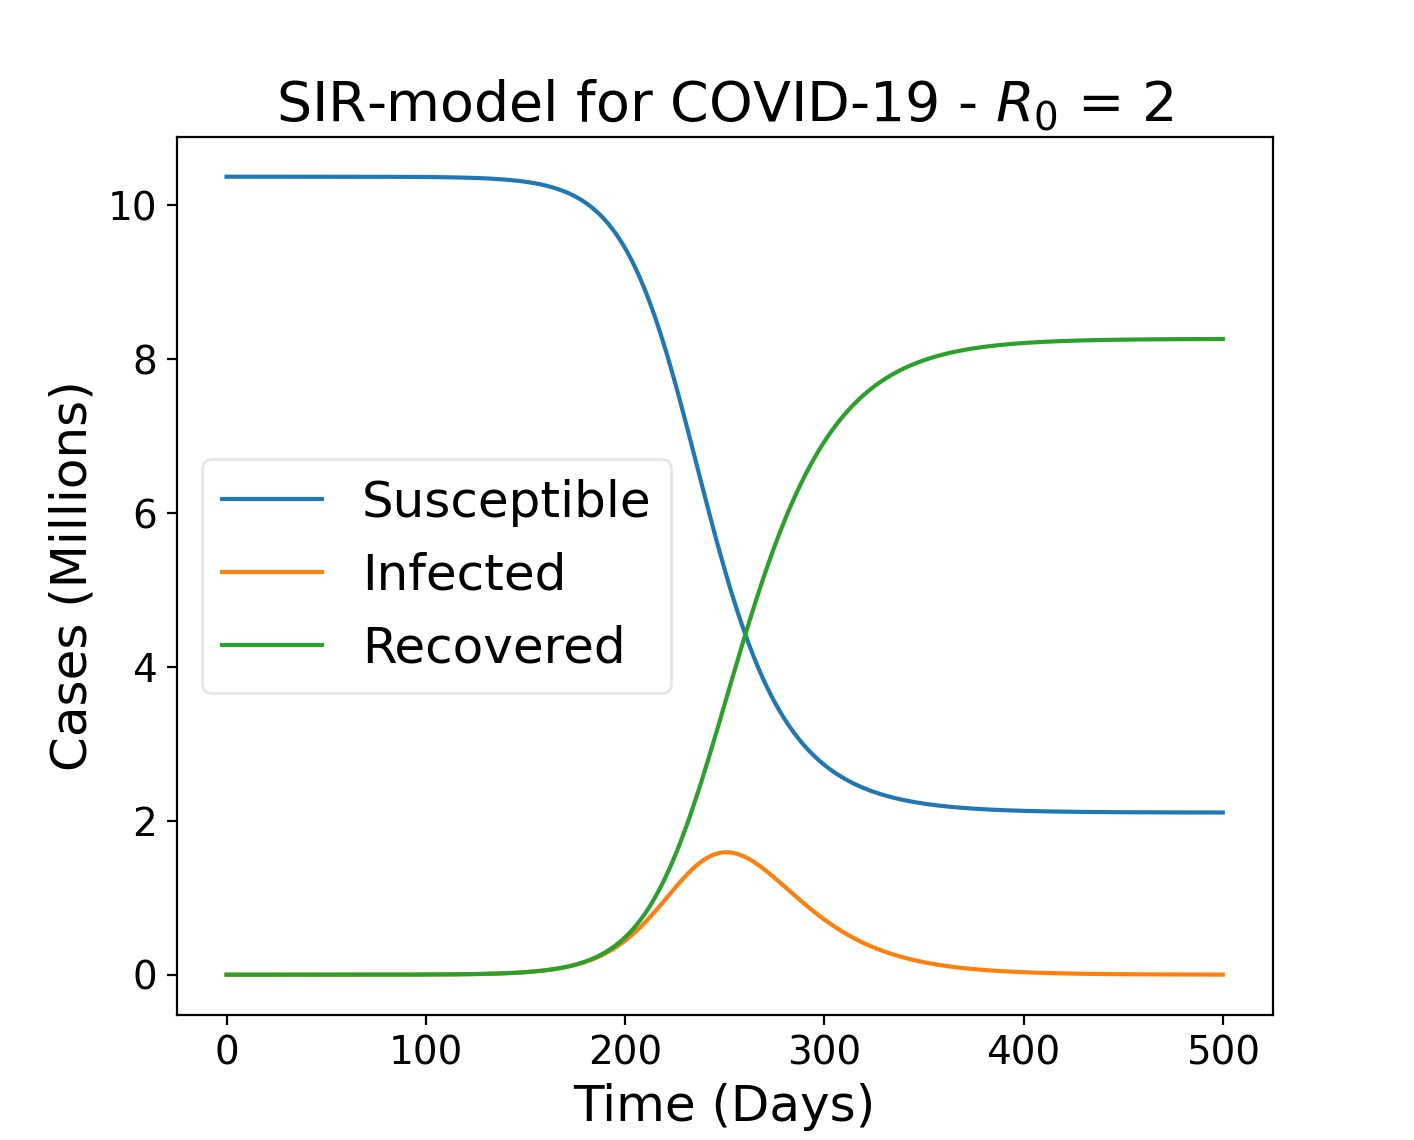
\includegraphics[width=0.45\textwidth]{SIR2.jpg}}
   \subfloat[\label{pyramidprocess}]{%
      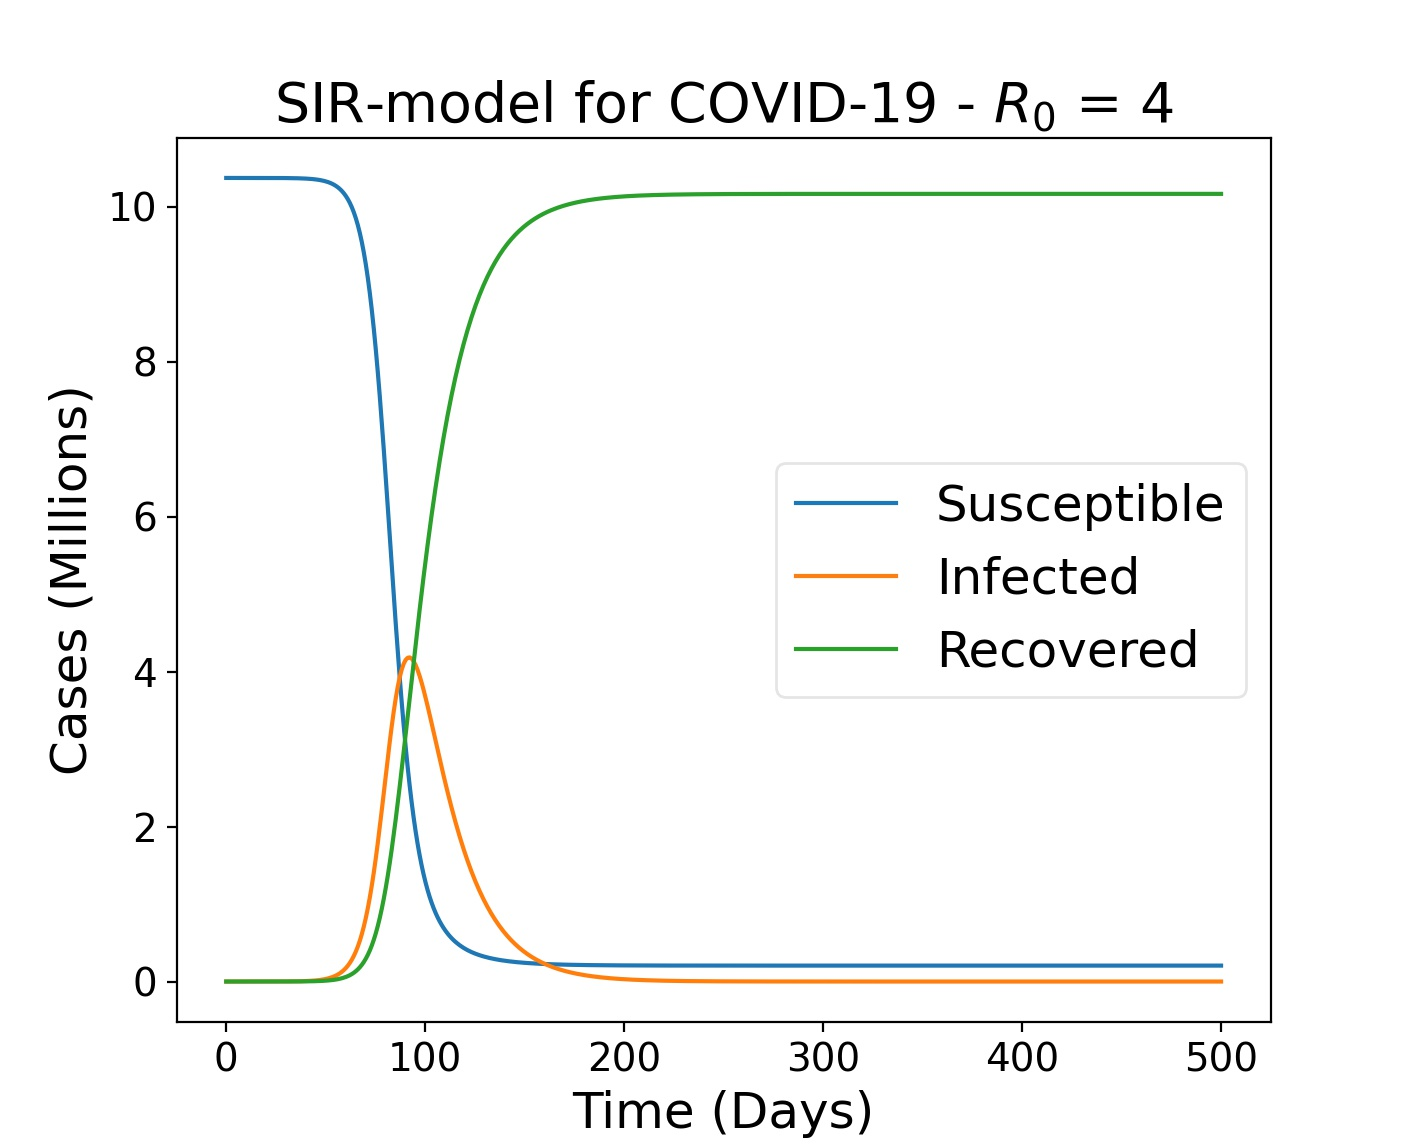
\includegraphics[ width=0.45\textwidth]{SIR4.jpg}}\\
   \caption{\label{workflow} (a) $R_0 = 2$, $\gamma = 1/18$ (b) $R_0 = 4$, $\gamma = 1/18$}
\end{center}
\end{figure*}
\subsection{SEIR - Comparisons for $R_0$-rates}
\begin{figure*}[ht!]
\begin{center}
   \subfloat[\label{genworkflow}]{%
      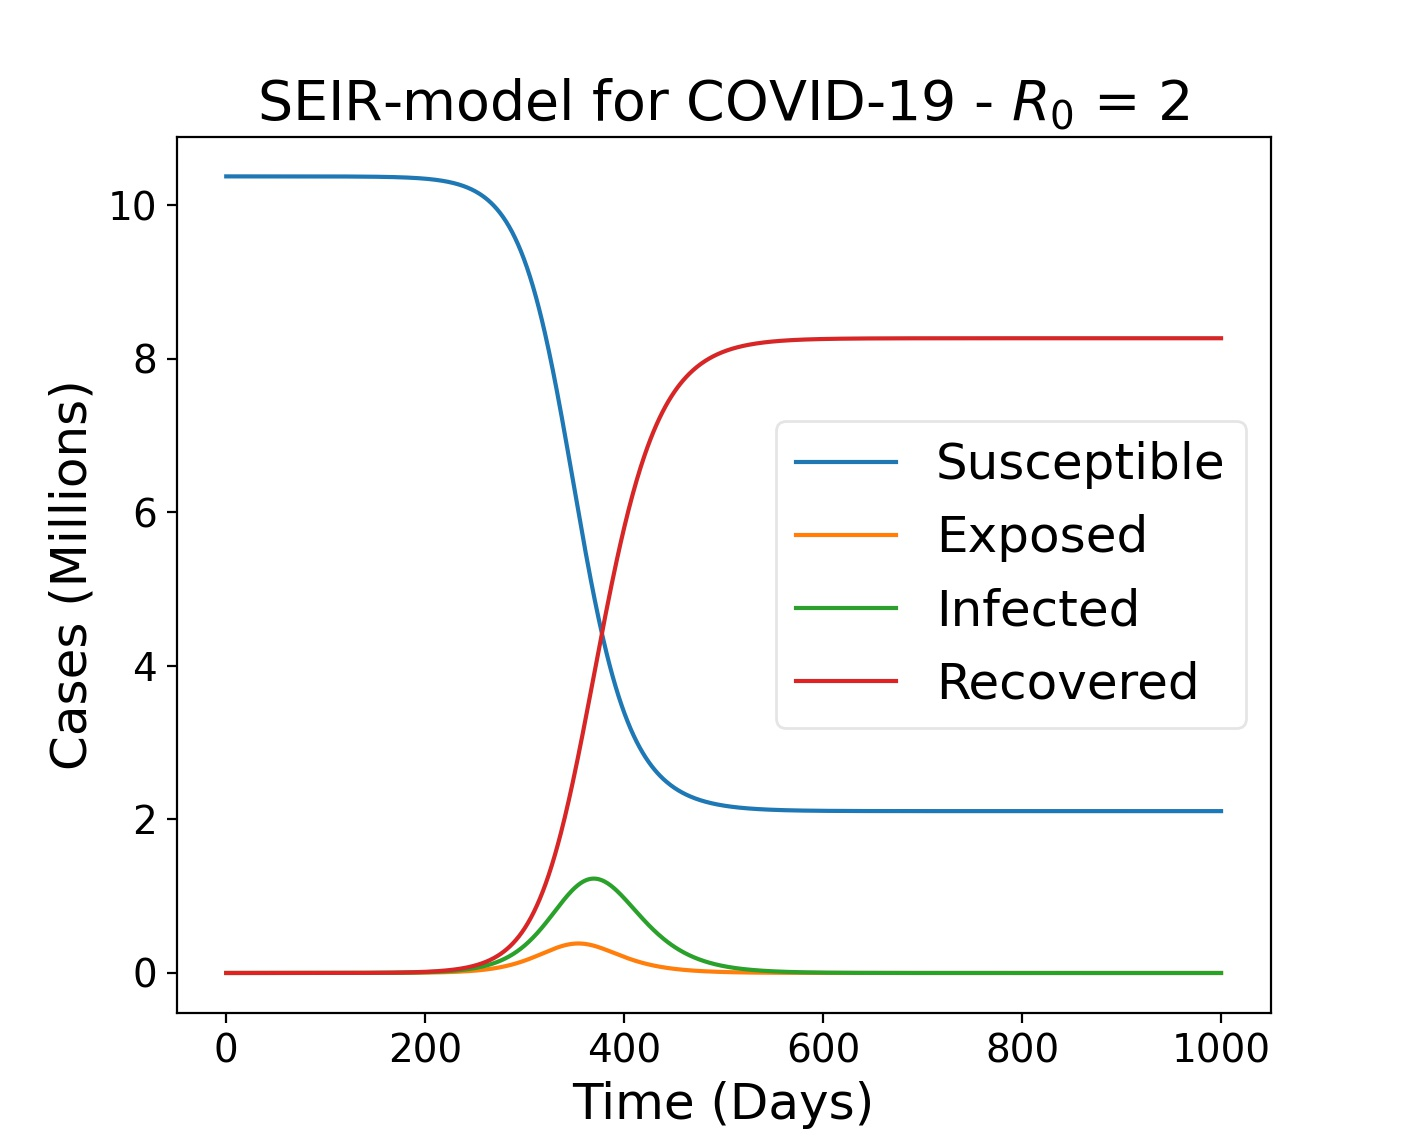
\includegraphics[width=0.45\textwidth]{SEIR2.jpg}}
   \subfloat[\label{pyramidprocess}]{%
      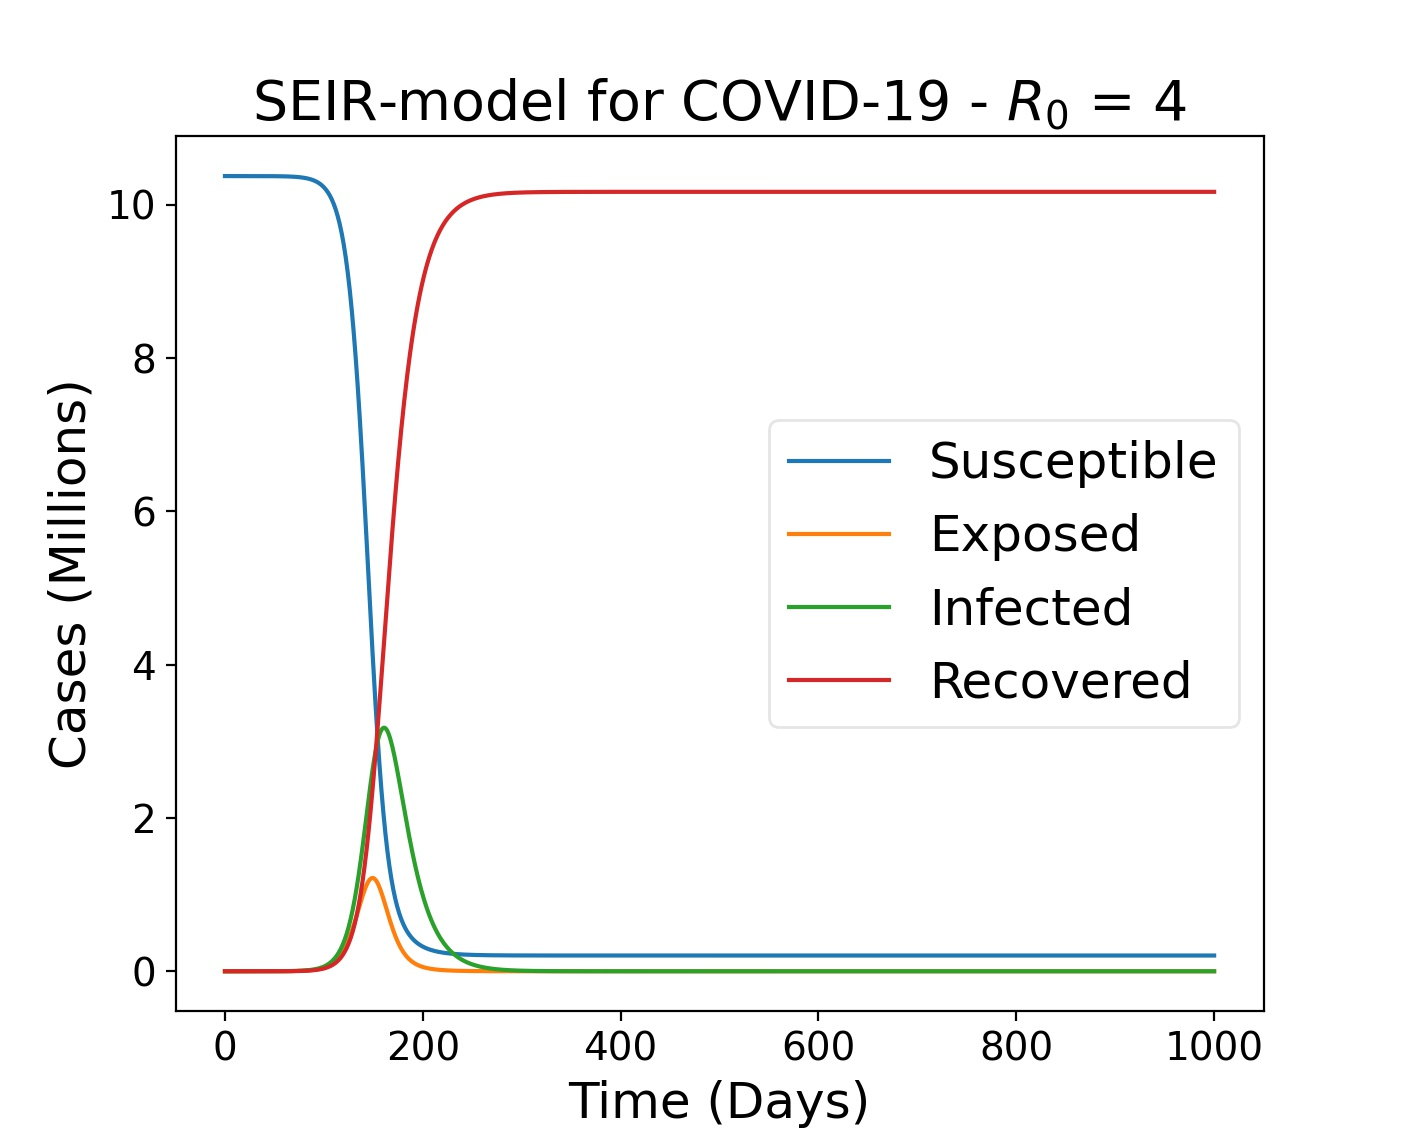
\includegraphics[ width=0.45\textwidth]{SEIR4.jpg}}\\
   \caption{\label{workflow} (a) $R_0 = 2$, $\alpha = 1/5.2$, $\gamma = 1/18$ (b) $R_0 = 4$, $\alpha = 1/5.2$, $\gamma = 1/18$}
\end{center}
\end{figure*}
\subsection{Analysis of the SIR and SEIR-models}
As for the epidemic SIR-model, it can be concluded that larger reproduction numbers result in more pervasive pandemics. Peak infections occur earlier and with larger populations. For smaller $R_0$ values
the progression of the pandemic follows a more gradual path, however with less serious consequences, i.e. infections and fatalities. 

For the SEIR-model, it can be concluded that the dependence on the reproduction number follows a similar pattern as to its SIR counterpart. However, the progressions of the outbreaks are more gradual due to infections having an incubation time.

\subsection{Phase space diagrams}
\begin{figure*}[ht!]
\begin{center}
   \subfloat[\label{genworkflow}]{%
      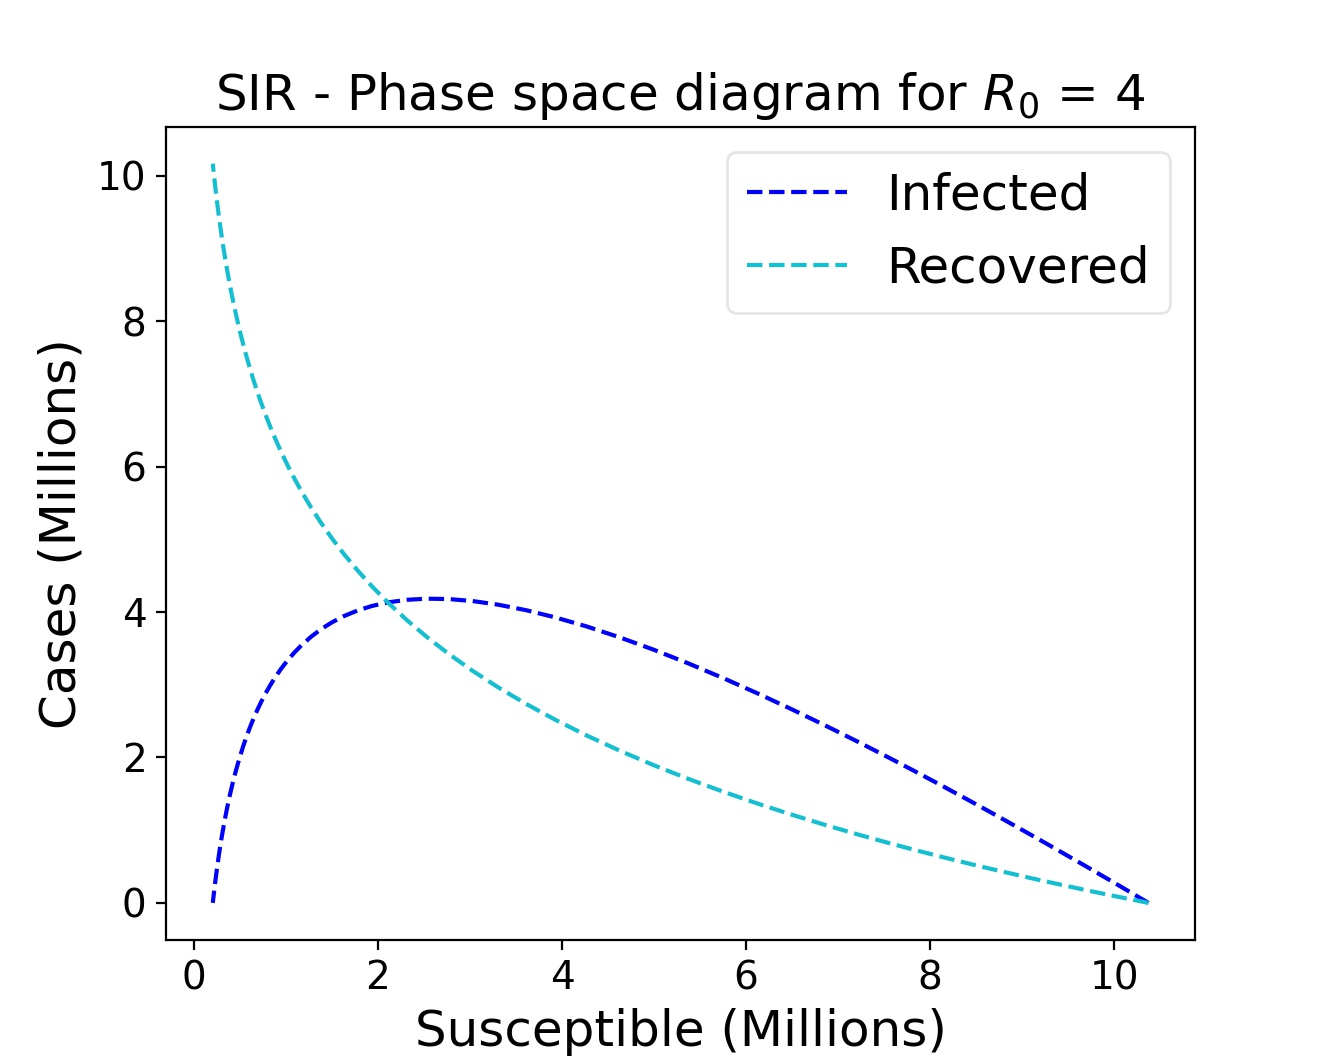
\includegraphics[width=0.45\textwidth]{SpaceSIR4.jpg}}
   \subfloat[\label{pyramidprocess}]{%
      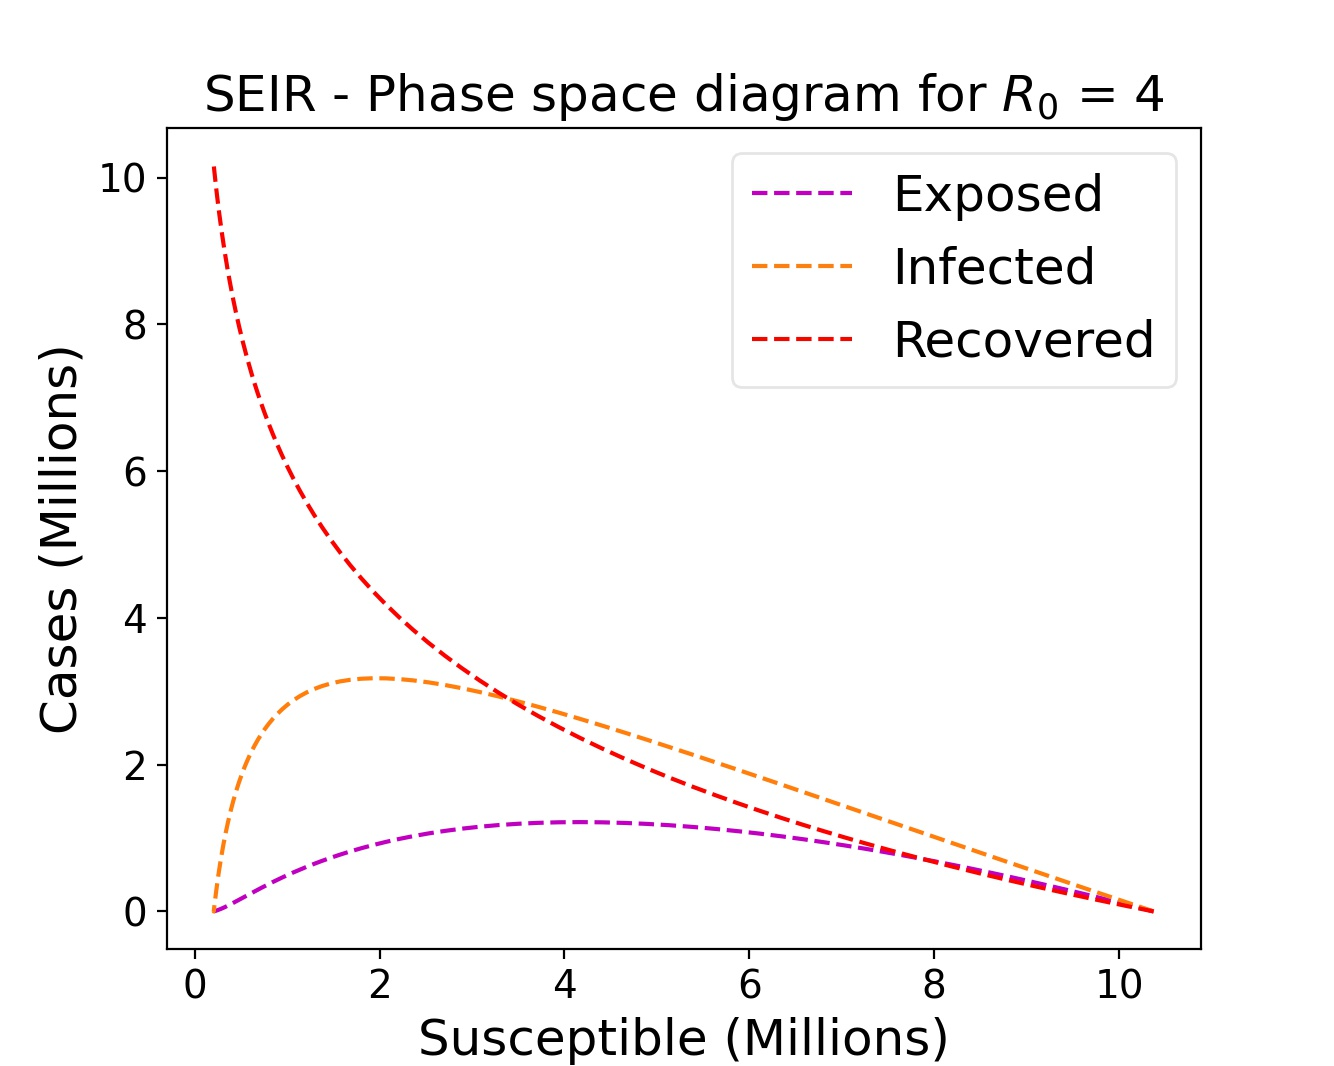
\includegraphics[ width=0.45\textwidth]{SpaceSEIR4.jpg}}\\
   \caption{\label{workflow} (a) SIR - $R_0 = 4$ (b) SEIR - $R_0 = 4$}
\end{center}
\end{figure*}
\noindent For both models, it can be concluded that an increase in the susceptible population increases in infected cases, while the recovered populations decrease as the susceptible decrease. 

The exposed population in the SEIR-model follows the same correlation as infected, however with a more marginal behavior. This also results in the infected population correlation in the SEIR-model being more gradual, which is attributed to the fact that the sum of these should add up to the infected population of the SIR-model.

\newpage 
\subsection{Implication of social distancing}
In order to analyze the implication of social distancing, 
a social distancing factor $\rho \in [0,1]$ can be introduced upon the SEIR-model \cite{gill}. As such, equations (2) summarize to:

\begin{gather}
\frac{dS}{dt} = - \frac{\rho \beta I S}{N} \;, \qquad
\frac{dE}{dt} = \frac{\rho \beta I S}{N}- \alpha E \;.
\end{gather}
One may note that in the case when $\rho = 1$, equations (6) are equivalent to equation (2) and this signifies no social distancing involved. By plotting the infected cases and fraction of  the susceptible population and varying $\rho$, the following diagrams are obtained.

\begin{figure*}[ht!]
\begin{center}
   \subfloat[\label{genworkflow}]{%
      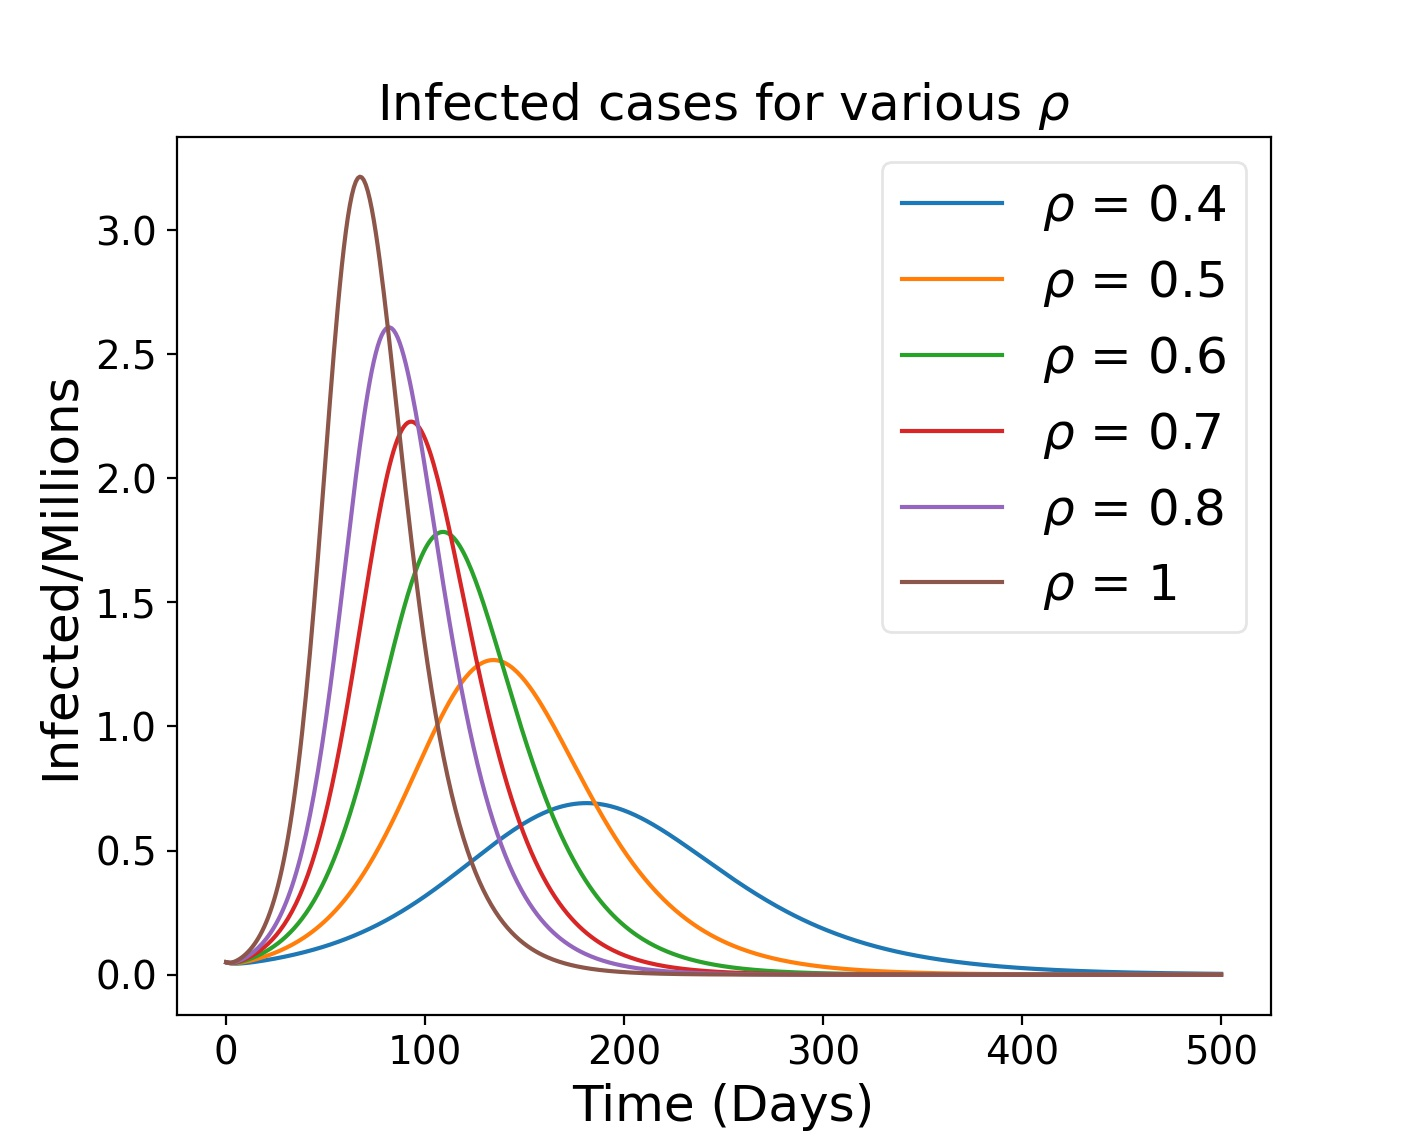
\includegraphics[width=0.45\textwidth]{Lockdown.jpg}}
   \subfloat[\label{pyramidprocess}]{%
      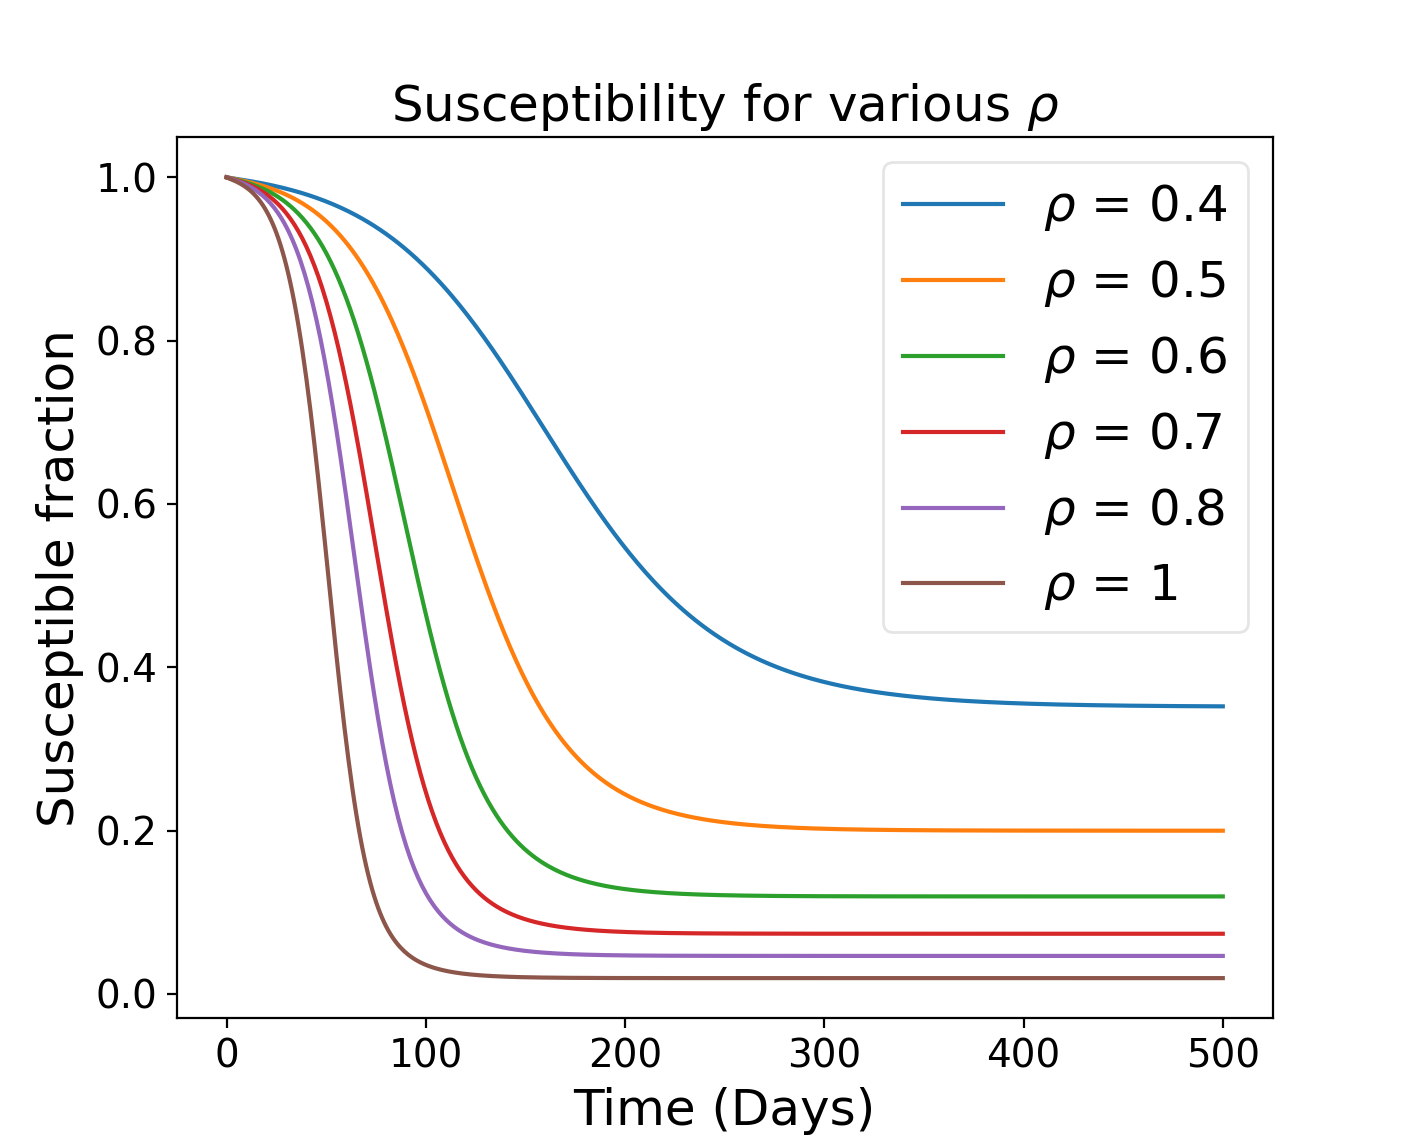
\includegraphics[ width=0.45\textwidth]{Susceptibility.png}}\\
   \caption{\label{workflow} (a) Infected cases (b) Susceptibility fraction}
\end{center}
\end{figure*}

\noindent As can be noted, higher levels of social interactions cause higher peaks for the infected populations as well as the peaks occurring earlier. This can have severe implications such as overwhelming the healthcare capacity. Lesser levels of social distancing prolong the duration of the pandemic, however with less serious repercussions. 
This phenomenon is commonly referred to as \textit{flattening the curve}.

The fraction of the susceptible population decreases as more time passes and decreases more rapidly for higher levels of social interactions. 
\newpage 
\noindent This is attributed to the higher number of infected individuals for larger $\rho$. One may also note that due to this decrease in the susceptible population, a later termination of lockdown measure would result in a lower peak for a resurgent \textit{second wave} and vice versa.

\subsection{Implication of vaccination}
In order to analyze the implication of vaccination in a population, the proportion of vaccinated population can be introduced upon the SIR model utilizing initial conditions:
\begin{equation}
S(0) = (1-p)(N-1), \; R(0) = p(N-1),  
\end{equation}
for $S$ and $R$ \cite{ashraf}. Note that as $p = 0$, equation (2) is identical to (7) which holds true when no vaccinations are implemented. 

\begin{figure*}[ht!]
\begin{center}
   \subfloat[\label{genworkflow}]{%
      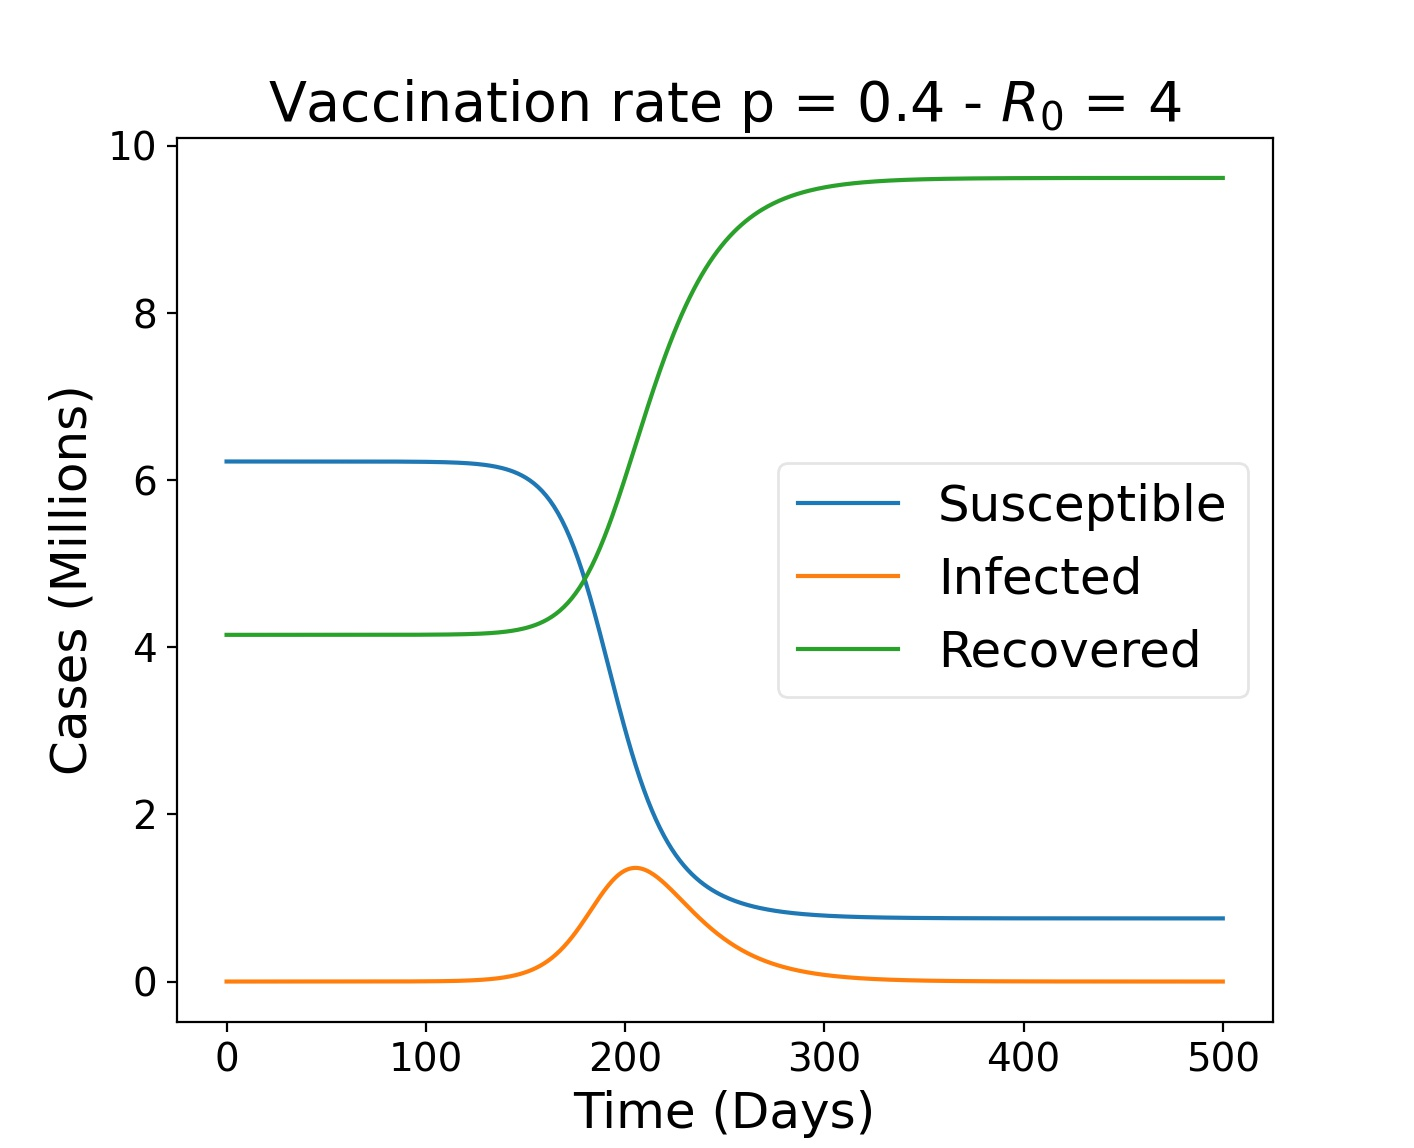
\includegraphics[width=0.45\textwidth]{Vaccination04.jpg}}
   \subfloat[\label{pyramidprocess}]{%
      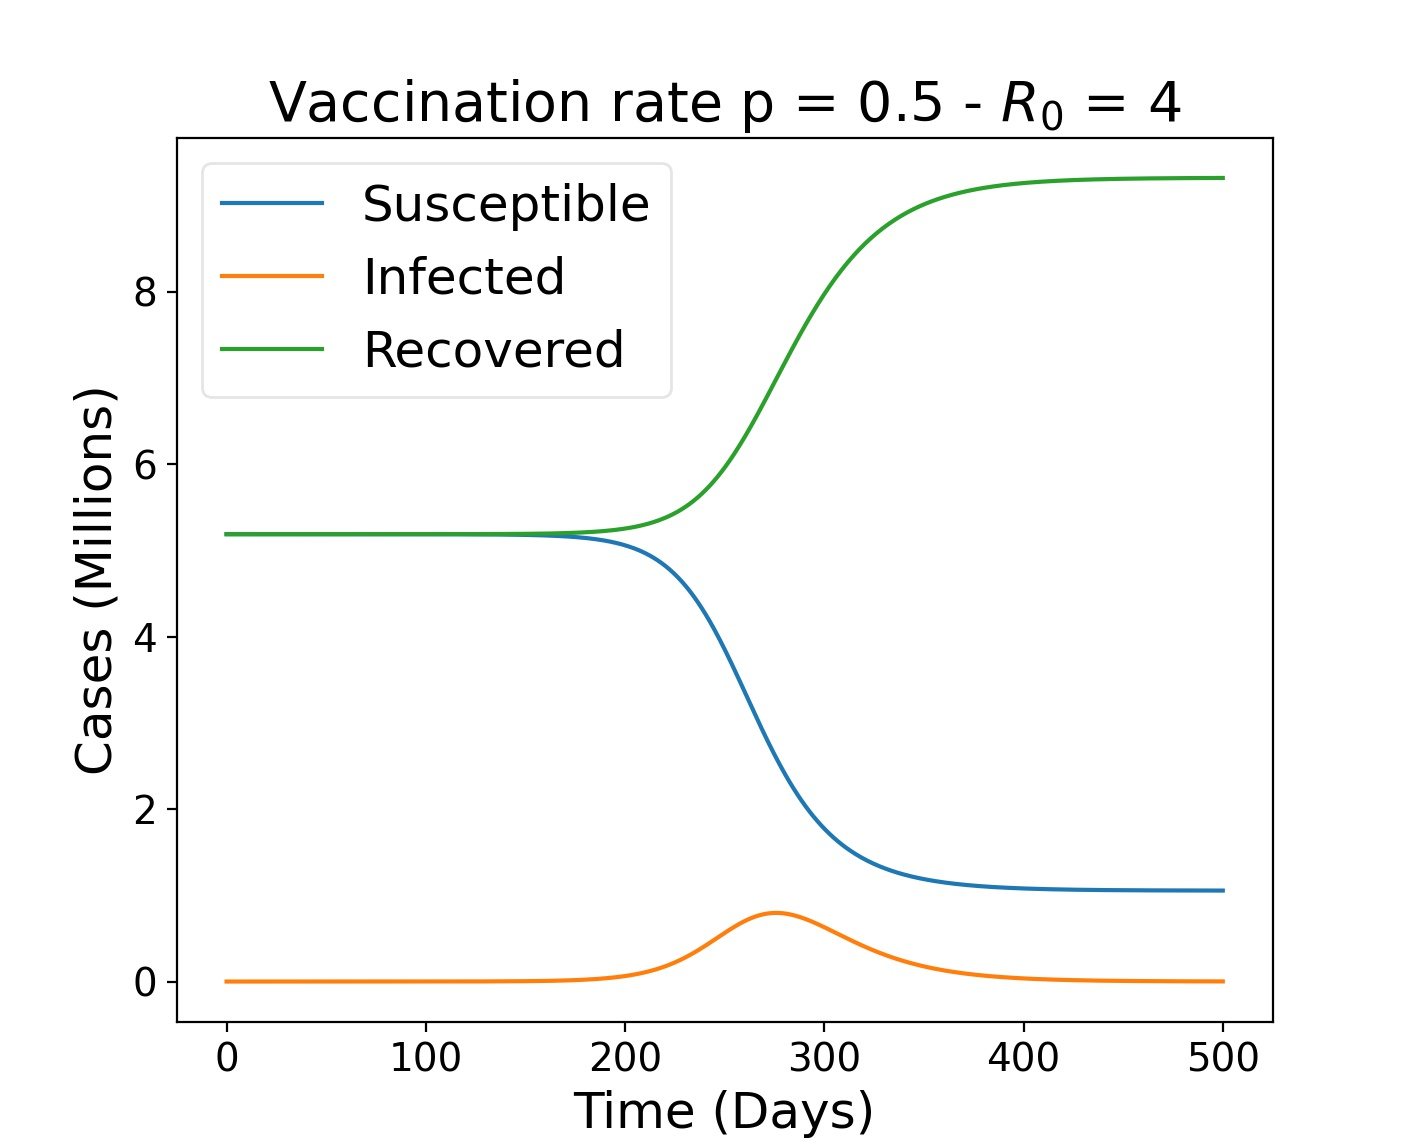
\includegraphics[ width=0.45\textwidth]{Vaccination05.jpg}}\\
   \caption{\label{workflow} (a) 40 \% vaccination rate (b) 50 \% vaccination rate}
\end{center}
\end{figure*}
\noindent As can be noted, the diagrams for $p = 0$ should be identical to Figure 1b and as the vaccination rate increases, the peak in infected individuals lessens and patients recover earlier. As in previous cases, the pandemic resolves more gradually but with less serious repercussions.

\section{Discussion}
\subsection{SIR and SEIR models}
As the reproduction number increases, the more infectious a disease is and causes a larger degree of devastation. It can also be concluded that the SEIR-model is more gradual compared to epidemic SIR and thus more realistically modeling an outbreak. By having only two parameters, the SIR model allows for simple predictions of disease behavior but this simplicity is also its main constraint. 

The SIR model does not consider incubation time, i.e. the period in which an individual becomes infected but not contagious. SEIR does however take account of this parameter but additional extensions are required to model in order more desirably match reality. Such extensions are for instance vital dynamics (endemic) and modeling of time-dependent mitigation measures but for simplicity's sake, these have been omitted. However, since pandemics at most times involve quick measures and recovery, vital dynamics have a more minor impact. 

Both models make various assumptions, assuming a homogeneous mixing of the population, a closed population as well as equal contact and transmission rates for all individuals in society. One would note that the social structures of humans are far more complex and as previously stated, many more factors must be taken into account. Closed populations, however, can be presumed as of the current day considering the imposed travel restrictions in most countries. 

Assumptions are also made in quantifying the parameters, with them only being rough estimations and may vary considerably for populations. This constraint and lack of precision could be alleviated by utilizing distributions for the parameters and thus simulating possible futures.

Finally, one must note that the SIR and SEIR models should only be interpreted as suggestive predictions of the outbreak and when different mathematical models yield qualitatively considerably different results, one may question some assumptions and deduce their inefficiencies. Nonetheless, even a moderately qualitative approximation can be highly useful for informing policymakers.


\newpage 

\subsection{Social distancing}
It can be noted that social distancing measures are highly effective at curbing the severity of the outbreak and once such mandates are terminated, one would expect a quick resurgence. Longer lockdowns result in less severe second waves due to a decrease in susceptible population over time. This phenomenon can be interpreted as \textit{herd immunity} and even though more social interaction (greater $\rho$-values) results in a smaller susceptible population, more fatalities and devastation will occur as compared to the more gradual progression for less social interactions (lesser $\rho$-values).
\subsection{Vaccination}
Just as social distancing, vaccination is also an effective measure in restraining a pandemic and could even be considered to be more desirable due to individuals becoming immune and falling into the \textit{Recovered} segment immediately. However vaccines take time to develop and do not appear at an instant. One should also note that there is no need for all individuals in a population to be vaccinated and this phenomenon can once again be attributed to \textit{herd immunity}. \textit{Herd immunity} in this case is attained when a sufficient proportion of the population is immune and thus not prone to furthering the transmission.

The proportion of vaccinated population required for basic \textit{herd immunity} can be represented by the formula: 
\begin{equation}
p_c = 1- \cfrac{1}{R_0},
\end{equation}
with $R_0$ being the reproduction number \cite{ashraf}. For COVID-19 with $R_0$ falling in the range of $2-6$, this proportion should fall between $50 \% - 83.3 \%$ of the population. This corresponds well with Figure 5, where the outbreak essentially dwindles at an approximate $8$ million recovered population. 
\newpage 
\subsection{Statistical accuracy}
As previously stated, the analytical solution for the SIS-model will be compared with the solutions generated by the aforementioned numerical integrators. The analytical solution for the SIS-model is given as:

\begin{equation}
\cfrac{(1-\gamma/\beta)N}{1+(\frac{(1-\gamma/\beta)N}{I_0}-1)
e^{-(\beta-\gamma)t}},  
\end{equation}
which can be derived by making a transformation of variables \cite{levin}.
By plotting the absolute differences between the numerical and analytical solutions for variables $S$ and $I$, the following diagrams were obtained.

\begin{figure*}[ht!]
\begin{center}
   \subfloat[\label{genworkflow}]{%
      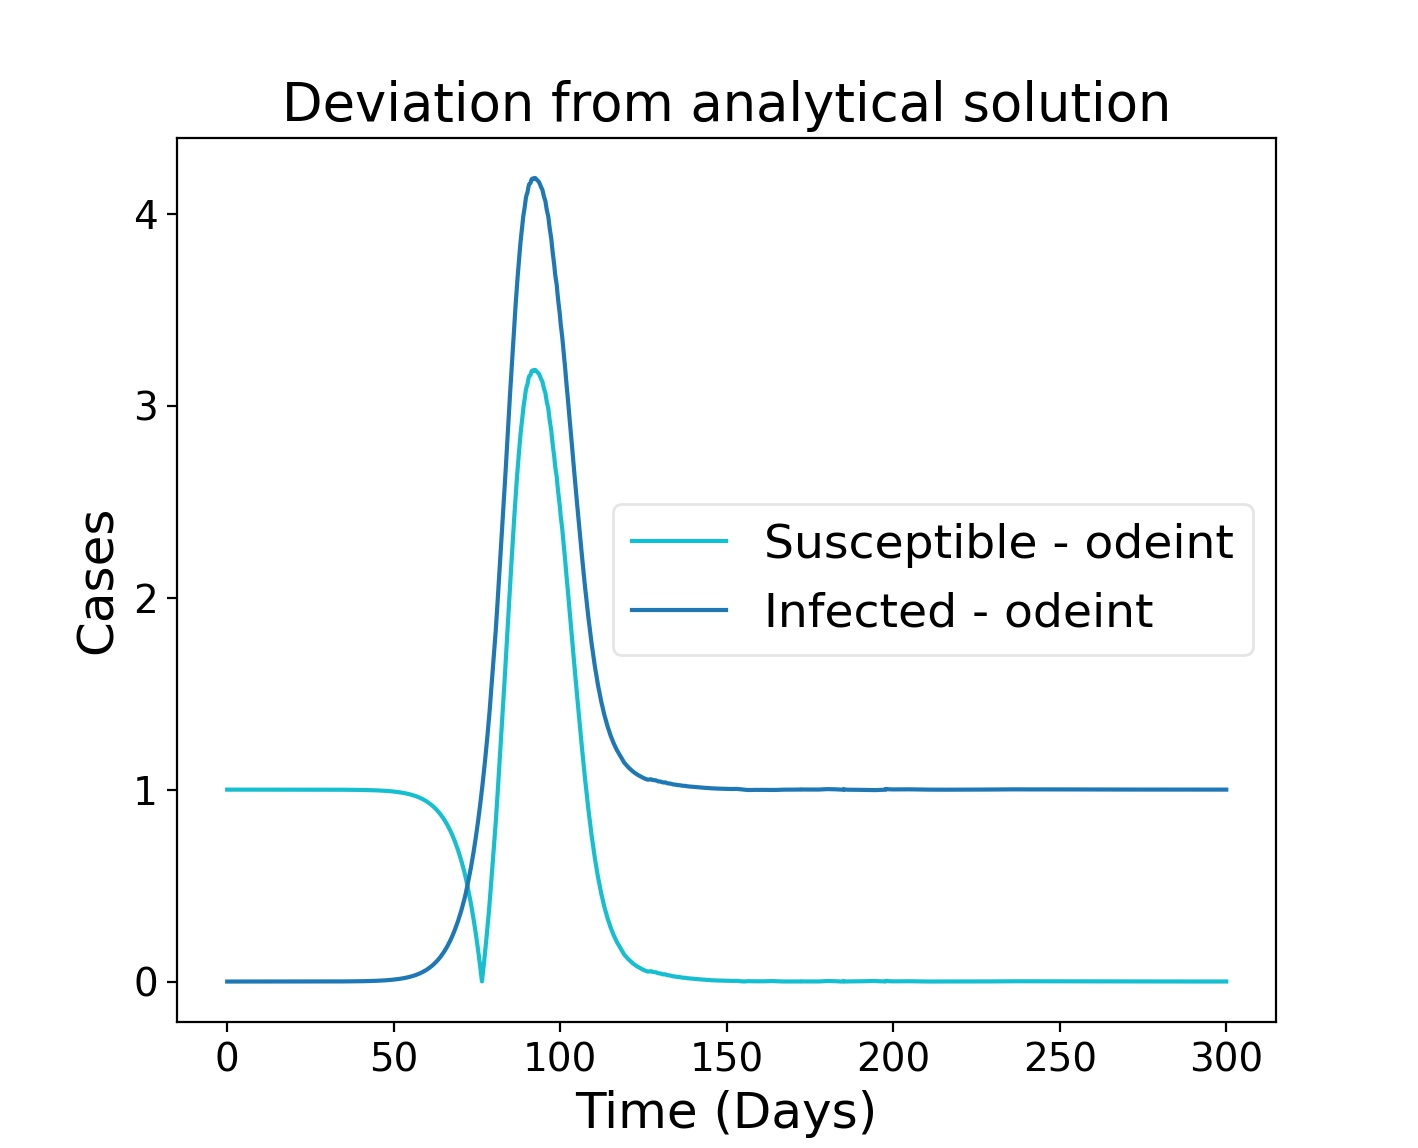
\includegraphics[width=0.45\textwidth]{odeint.jpg}}
   \subfloat[\label{pyramidprocess}]{%
      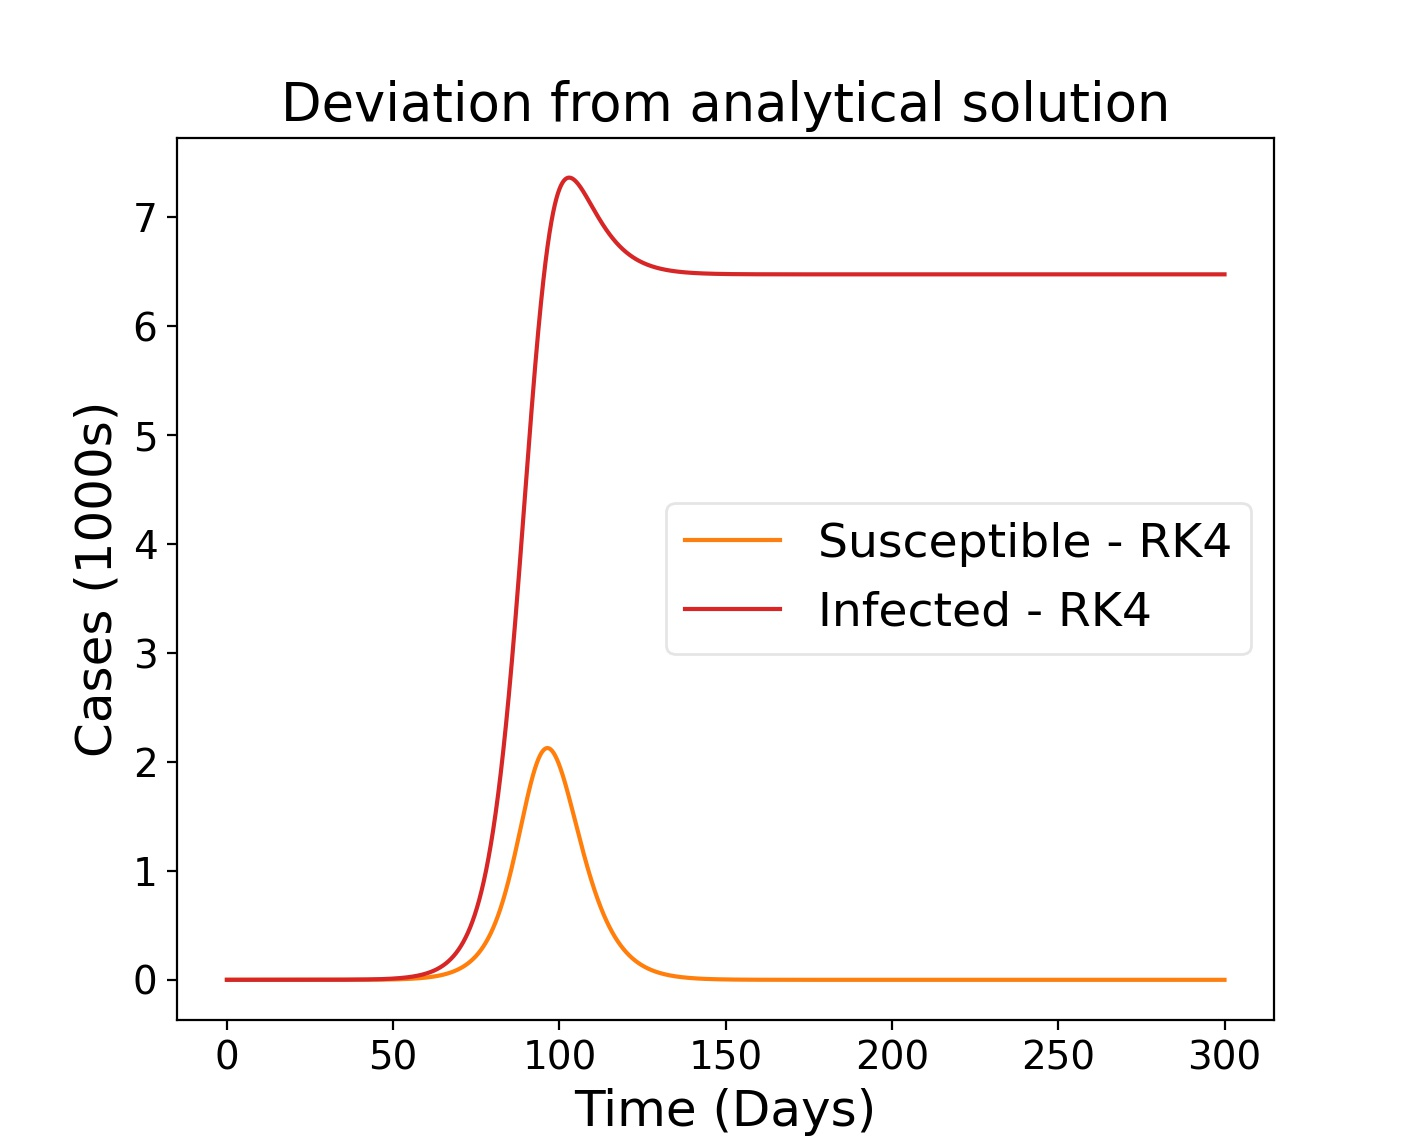
\includegraphics[ width=0.45\textwidth]{RK4h001.jpg}}\\
   \caption{\label{workflow} (a) Error margin for $odeint$ (b) Error margin for  RK4 - $h = 0.01$}
\end{center}
\end{figure*}
\noindent As can be noted, $odeint$ yields far more exact results than the fourth order RK4 with step size $h = 0.01$ and that is the overwhelming reason for using it as the preferred numerical integrator. For large populations such as in this case, the magnitude difference is negligible and the two integrators both yield qualitative results. However, for smaller populations sizes, $odeint$ will undoubtedly outshine its counterpart. 

Despite having peak deviations, both methods approximate the susceptible population better than the infected population, attributing to the fact that they converge towards the analytical solution (deviation of 0) for long times. 
\newpage 
\noindent As for the susceptible populations, both methods show an immature increase in value and converging for longer times, however not towards the analytical solution. Despite the fact that RK4 for the given step size does not attain the same precision as $odeint$, the step size can be further incremented. For $h = 0.001$ and $h = 0.0001$, the following error margins were to be observed.
\begin{figure*}[ht!]
\begin{center}
   \subfloat[\label{genworkflow}]{%
      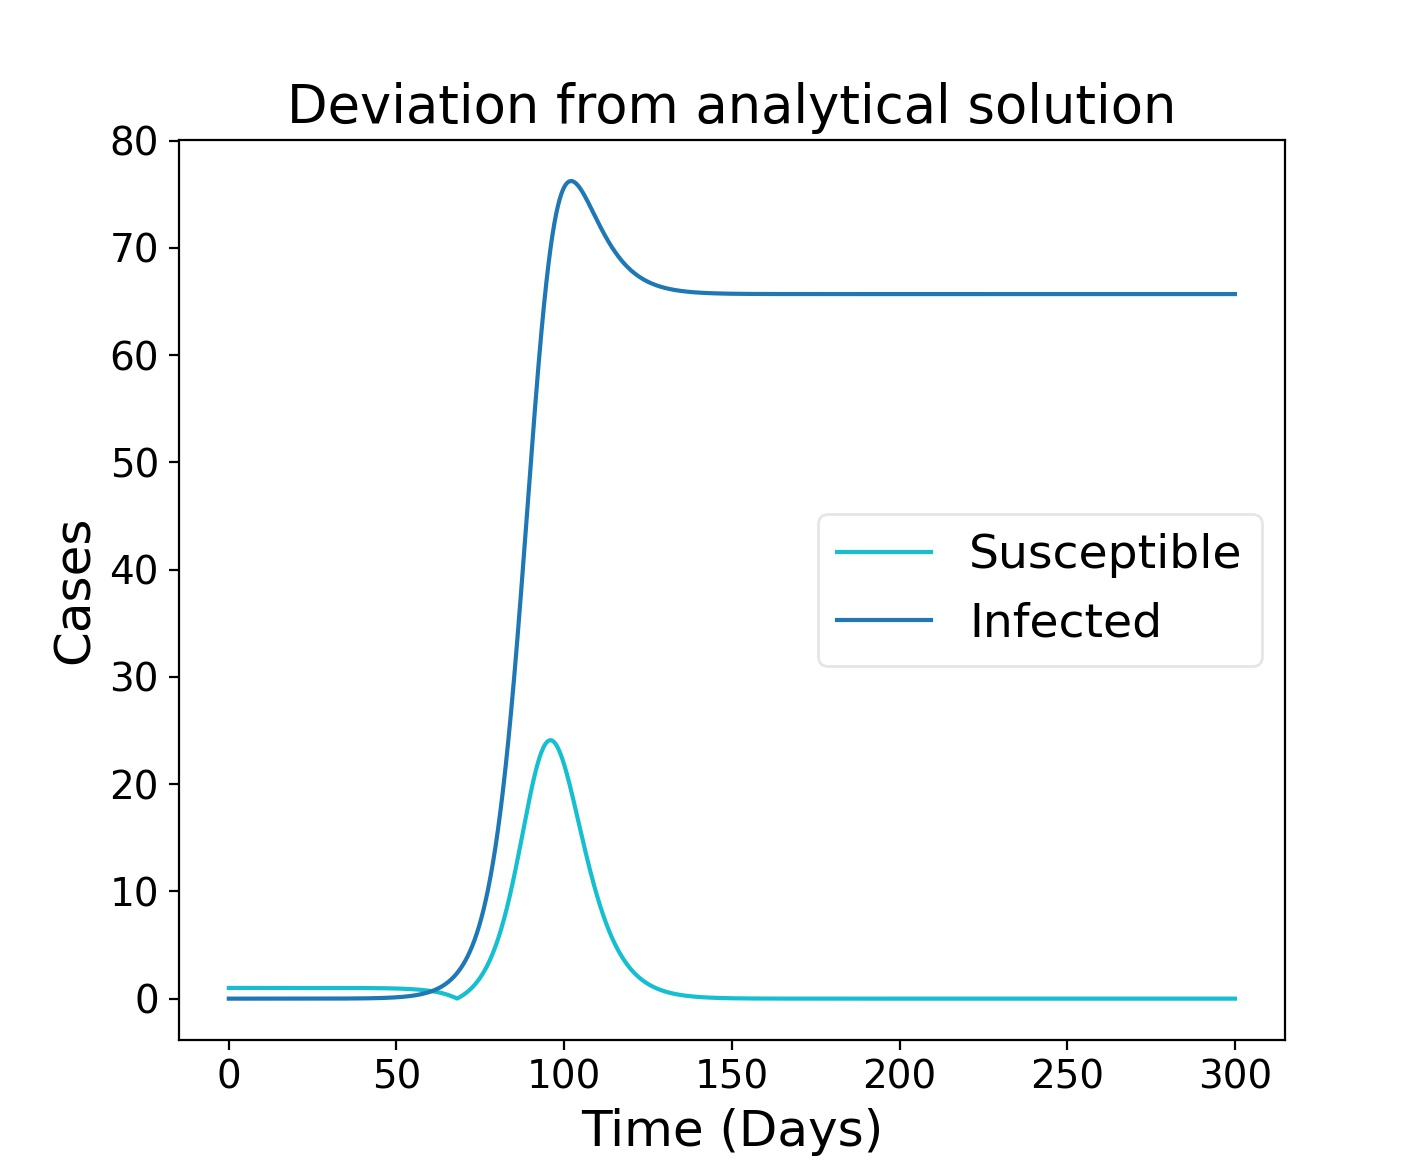
\includegraphics[width=0.45\textwidth]{RK4h00001.jpg}}
   \subfloat[\label{pyramidprocess}]{%
      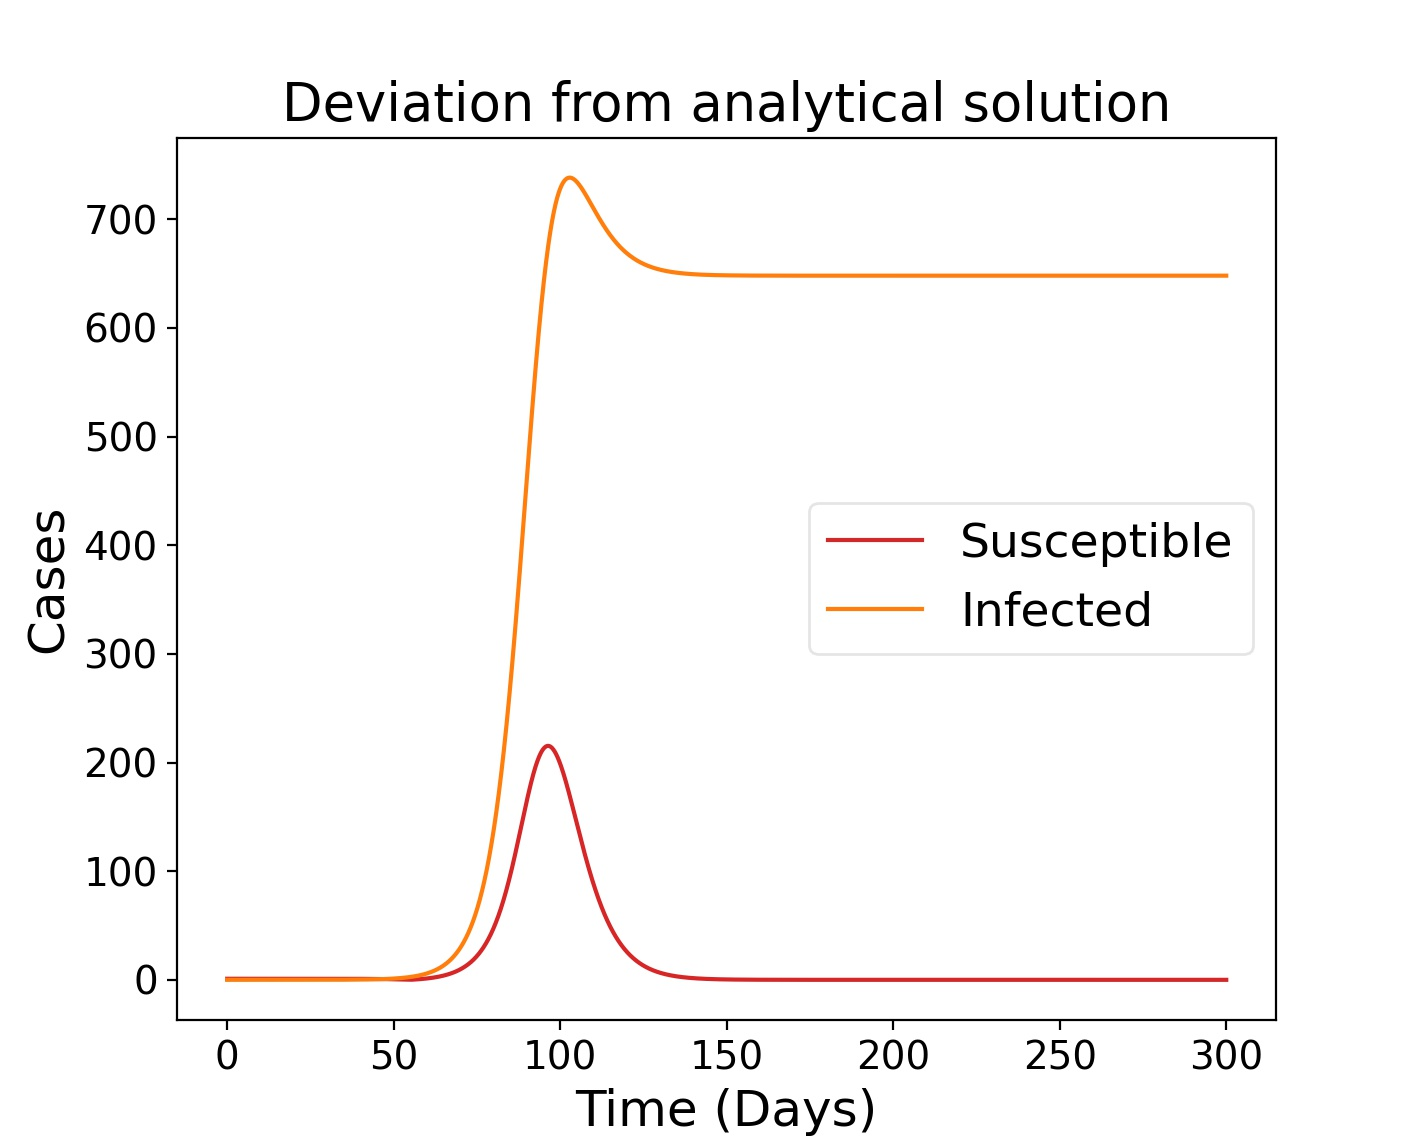
\includegraphics[width=0.45\textwidth]{RK4h0001.jpg}}\\
   \caption{\label{workflow} (a) RK4 - $h = 0.0001$ (b) RK4 - $h = 0.001$}
\end{center}
\end{figure*}

\noindent As can be noted from the diagrams, the error margin for RK4 decreases for smaller step sizes and should attain the same magnitude as in $odeint$ and be comparably precise. However, this comes at the expense of the computational time, with $odeint$ being considerably faster for margins of error of the same magnitudes. 

According to the Scipy library, there is no simple description of the algorithmic complexity of $odeint$, which is based on an $lsoda$ integrator from FORTRAN. The $lsoda$ integrator alternates between a stiff BDF and non-stiff Andrews method, which changes step size in accordance with internal error estimates \cite{scipy}.  This should be the primary reason for the precise and qualitative behavior shown by $odeint$ in solving the compartmental models. 

\newpage
\section{Conclusions}
It can be concluded that the SIR and SEIR are simplified representations of reality and due to this simplification, a huge amount of constraints are bestowed upon them. Although being so uncomplicated, the compartmental model does an excellent job in giving a rough approximation of possible outcomes of an outbreak, with SEIR being the more realistic of them. The compartmental models are highly flexible so by introducing more parameters and variables, they should better correspond to reality. 

One could also note that terms such as \textit{herd immunity} and \textit{flattening} the curve may initially seem vague but with mathematical visualizations, these phenomena can be simulated by varying the parameters. As such computer simulations and mathematical modeling are powerful tools in assessing the outcomes of various phenomenons in reality. 
  
The SARS-CoV-2-virus has spread extremely hastily and the COVID-19 pandemic is often compared to other recent pandemics, such as the SARS-outbreak in 2002-2004. Despite being less lethal, COVID-19 is much more infectious than SARS and that can be explained by comparing their reproduction numbers, with SARS falling within the range of 0.19-1.08 
\cite{chowell}. This demonstrates that by varying $R_0$, one could sufficiently assess the infectivity for various pathogens.

Some degree of chaotic behavior can be noted for both the SIR and SEIR models with and without modifications, considering that variation of the model parameters, $\alpha$, $\beta$, $\gamma$, $\rho$ could result in substantial alterations for the  $S$ and  $I$ trajectories if large enough. However, the effect is not substantial for small variations and thus it can be argued that the models are not chaotic in nature.

As for the numerical integrators, it can be included that both $odeint$ and the fourth-order Runge-Kutta methods yield qualitative approximations for the analytical solutions, with $odeint$ having an advantage over its counterpart. RK4 has a constant but high order accuracy of $O(h^5)$ but from the simulations, it seemingly appears that constantly altering the order accuracy for internal error estimates is a more effective course of action. Although no order accuracies for the $odeint$ are listed, it can be concluded that it should be higher than RK4 for some instances.
 
\newpage 
\section{References}
\printbibliography[heading=none]
\end{document}
